\PassOptionsToPackage{table}{xcolor}
\documentclass{beamer}
%\documentclass[handout]{beamer}

\setbeamertemplate{bibliography item}{\insertbiblabel}

\usepackage[utf8]{inputenc}
\usepackage{algorithm, algorithmic}
\usepackage{caption}
\usepackage{mathtools}
\usepackage{tabularx}
\usepackage{color, colortbl}
\usepackage{array, booktabs, ragged2e}
\usepackage{makecell}
\usepackage{tikz}
\usepackage{textpos}

\definecolor{RowColorOdd}{rgb}{0.914,0.914,0.953}
\definecolor{RowColorEven}{rgb}{1,1,1}

\definecolor{lightgray}{rgb}{0.83, 0.83, 0.83}

\renewcommand\theadfont{\bfseries}

\usepackage[backend=biber]{biblatex}
\addbibresource{References.bib}

\DeclareMathOperator{\balance}{balance}
\DeclareMathOperator{\argmin}{argmin}

\renewcommand*{\bibfont}{\tiny}

\usetheme{Madrid}
\usecolortheme{default}

%------------------------------------------------------------
%This block of code defines the information to appear in the
%Title page
\title[Fair Clustering Through Fairlets]
{Fair Clustering Through Fairlets}

\subtitle{(EE531 Final Project - Fairness)}

\author[Junghyun Lee]
{F.~Chierichetti\inst{1} \and R.~Kumar\inst{2} \and S.~Lattanzi\inst{2} \and S.~Vassilvitskii\inst{2}}

\institute[KAIST]
{
	\inst{1}%
	Dipartimento di Informatica,
	Sapienza University
	
	\inst{2}%
	Google Research
}

\date[NIPS 2017]
{Appeared at NIPS 2017}


%End of title page configuration block
%------------------------------------------------------------



%------------------------------------------------------------
%The next block of commands puts the table of contents at the 
%beginning of each section and highlights the current section:

\AtBeginSection[]
{
  \begin{frame}
    \frametitle{Outline}
    \tableofcontents[currentsection]
  \end{frame}
}

\AtBeginSubsection[]
{
  \begin{frame}
    \frametitle{Outline}
    \tableofcontents[currentsection, currentsubsection]
  \end{frame}
}
%------------------------------------------------------------


\begin{document}

%The next statement creates the title page.
\frame{\titlepage}


%---------------------------------------------------------
%This block of code is for the table of contents after
%the title page
\begin{frame}
\frametitle{Table of Contents}
\tableofcontents
\end{frame}
%---------------------------------------------------------

\section{Introduction}

%---------------------------------------------------------
\begin{frame}
\frametitle{Disparate Impact}
\setbeamerfont{footnote}{size=\tiny}

\begin{itemize}
    \item {\bf Griggs v. Duke Power Co.}\footfullcite{Griggs1971}: the most significant U.S.S.C. rulings on disparate(or adverse) impact. \pause
    
    \item "Congress has now provided that tests or criteria for employment or promotion may-not provide equality of opportunity merely in the sense of the fabled offer of milk to the stork and the fox" \pause
    
    \item \alert{Disparate impact}: "substantially different rate of selection in hiring, promotion, or other employment decision which works to the disadvantage of members of a race, sex, or ethnic group"\footfullcite{uniform} \pause
    
    \item cf. $80\%$-rule\footfullcite{Biddle2006}
\end{itemize}
\end{frame}

%---------------------------------------------------------
\begin{frame}
\frametitle{Introduction}
\setbeamerfont{footnote}{size=\tiny}

\begin{itemize}
    \item In this work, the notion of \alert{disparate impact}, as described previously, will be followed! \pause
    
    \item Question: How can we formalize this notion of disparate impact in the case of clustering problem?
\end{itemize}
\end{frame}

%---------------------------------------------------------

\section{Previous / Related Works}

%---------------------------------------------------------
\begin{frame}
\frametitle{Previous / Related Works}
\setbeamerfont{footnote}{size=\tiny}

\begin{itemize}
    \item Two "big" tracks in fairness research:
    	\begin{itemize}
    		\item Codifying the meaning of fairness in algorithms
    		\item Modifying algorithms to make it achieve fair outcomes under a specific notion of fairness
    	\end{itemize} \pause
    
	\item In the case of disparate impact, Feldman {\it et al.}\footfullcite{Feldman2015} did some work in the first track. \pause
    
    \item This work is similar to the second track, but one of the first in the unsupervised learning tasks. \pause
    
    \item Unlike other works, {\it strong guarantees} on the quality of any fair clustering solution.
\end{itemize}
\end{frame}

%---------------------------------------------------------
\begin{frame}
\frametitle{Previous / Related Works}
\setbeamerfont{footnote}{size=\tiny}

\begin{itemize}
    \item The general framework of this work follows that of Zemel {\it et al.}\footfullcite{Zemel2013}. \pause
    
    \item Learn a set of intermediate representations to satisfy two competing goals: \pause
    \begin{itemize}
    	\item The intermediate representation should encode the data as well as possible.
    	\item The encoded representation is sanitized in the sense that it should be \alert{blind to whether or not the individual is from the protected group}.
    \end{itemize} \pause
    
    \item Using this, any classification algorithm can be transformed into a fair classifier, by simply {\it applying the classifer to the sanitized representation of the data}.
\end{itemize}
\end{frame}
%Namely, we formulate fairness as an optimization problem of finding an intermediate representation of the data that best encodes the data (i.e., preserving as much information about the individual’s attributes as possible), while simultaneously obfuscates aspects of it, removing any information about membership with respect to the protected subgroup. 

%---------------------------------------------------------
\begin{frame}
\frametitle{Previous / Related Works}
\setbeamerfont{footnote}{size=\tiny}

\begin{itemize}
    \item This work is also closely related to that of Zafar {\it et al.}\footfullcite{Zafar2017}. \pause
    
    \item Part of their work was focused on designing a convex margin-based classifier that maximizes accuracy subject to fairness constraints, and helps ensure compliance with a non-discrimination policy or law (e.g., a given $p\%$-rule) \pause
        
    \item This work addresses an open question in that work, which asked for a general framework to solve an unsupervised learning task respecting the $p\%$-rule.
\end{itemize}
\end{frame}
%In this paper, we introduced a novel measure of decision boundary fairness, which enables us to ensure fairness with respect to one or more sensitive attributes, in terms of both disparate treatment and disparate impact. We leverage this measure to derive two complementary formulations: one that maximizes accuracy subject to fairness constraints, and helps ensure compliance with a non-discrimination policy or law (e.g., a given p%-rule); and another one that maximizes fairness subject to accuracy constraints, and ensures fulfilling certain business needs (e.g., disparate impact’s business necessity clause).


%---------------------------------------------------------

\section{Preliminaries}

%---------------------------------------------------------
\begin{frame}
\frametitle{$k$-clustering}

\begin{block}{Definition}
Let $(M, d)$ be a metric space, equipped with the metric function $d$.

Given a set of points $X \subset M$, a {\it $k$-clustering} of $X$ is a partition of $X$ into $k$ disjoint subsets, $C_1, \dots, C_k$, called {\it clusters}.
\end{block} \pause

\begin{block}{Alternate Formulation}
A {\it $k$-clustering} of $X$ is an {\it assignment function}, $\alpha: X \rightarrow [k]$.

Each cluster $C_i$ is the preimage of $i$ under $\alpha$ i.e. $C_i = \alpha^{-1}(i)$
\end{block}

\begin{itemize} \pause
    \item There are many ways to quantify "how good a given clustering is"
    \item Depending on the objective, different variants of clustering problems are possible.
    \item Here, we consider two specific types of $k$-clustering.
\end{itemize}
\end{frame}

%---------------------------------------------------------


%---------------------------------------------------------
\begin{frame}
\frametitle{$k$-center problem}

\begin{block}{Problem}
Given a set of points $X \subset M$, find a $k$-clustering of $X$, denoted as $\mathcal{C}$, that minimizes
$$\phi(X, \mathcal{C}) = \max_{C \in \mathcal{C}} \left[ \min_{c \in C} \max_{x \in C} d(x, c) \right]$$
\end{block}
\end{frame}

%---------------------------------------------------------


%---------------------------------------------------------
\begin{frame}
\frametitle{$k$-median problem}

\begin{block}{Problem}
Given a set of points $X \subset M$, find a $k$-clustering of $X$, denoted as $\mathcal{C}$, that minimizes
$$\psi(X, \mathcal{C}) = \sum_{C \in \mathcal{C}} \left[ \min_{c \in C} \sum_{x \in C} d(x, c) \right]$$
\end{block}
\end{frame}

%---------------------------------------------------------


%---------------------------------------------------------
\begin{frame}
\frametitle{Fair clustering?}

\begin{itemize}
    \item In order to consider a "fair" version of clustering, we first have to identify the {\it unprotected attribute} and {\it protected attribute} \pause
    \item We shall consider the {\it coordinate} as the unprotected attribute. \pause
    \item For simplicity, let us represent the protected attribute as the {\it coloring} of the points. \pause
    \item To simplify things further (as in the paper), let us only consider the case of binary coloring.
\end{itemize}

\end{frame}

%---------------------------------------------------------


%---------------------------------------------------------
\begin{frame}
\frametitle{Fair clustering?}
For $Y \subset X$, let us denote:
\begin{itemize}
	\item $\chi : X \rightarrow \{\text{RED}, \text{BLUE}\}$ is the given binary coloring.
	\item $R(Y) = \{x \in X : \chi(x) = \text{RED}\}$, $r(Y) = |R(Y)|$
	\item $B(Y) = \{x \in X : \chi(x) = \text{BLUE}\}$, $b(Y) = |B(Y)|$ \pause
\begin{block}{Definition}
For $\emptyset \not= Y \subset X$, the {\it balance} of $Y$ is defined as:
$$\balance(Y) = \min \left( \frac{r(Y)}{b(Y)}, \frac{b(Y)}{r(Y)} \right) \in [0, 1]$$

The {\it balance} of a clustering $\mathcal{C}$ is defined as:
$$\balance(\mathcal{C}) = \min_{C \in \mathcal{C}} \balance(C)$$
\end{block}

	\item If $\balance(Y)$ is $0$(resp. $1$), $Y$ is fully unbalanced(resp. perfectly balanced)
\end{itemize}

\end{frame}

%---------------------------------------------------------


%---------------------------------------------------------
\begin{frame}
\frametitle{Fair clustering?}

\begin{itemize}
	\item A clustering algorithm is {\it colorblind} if it doesn't take the protected attribute (coloring) into its decision making. \pause
	\item Colorblind algorithm may result in a very unfair clustering.\\
	(Unfair in the sense that the resulting clustering is very unbalanced)
		\begin{figure}[hbt]
  			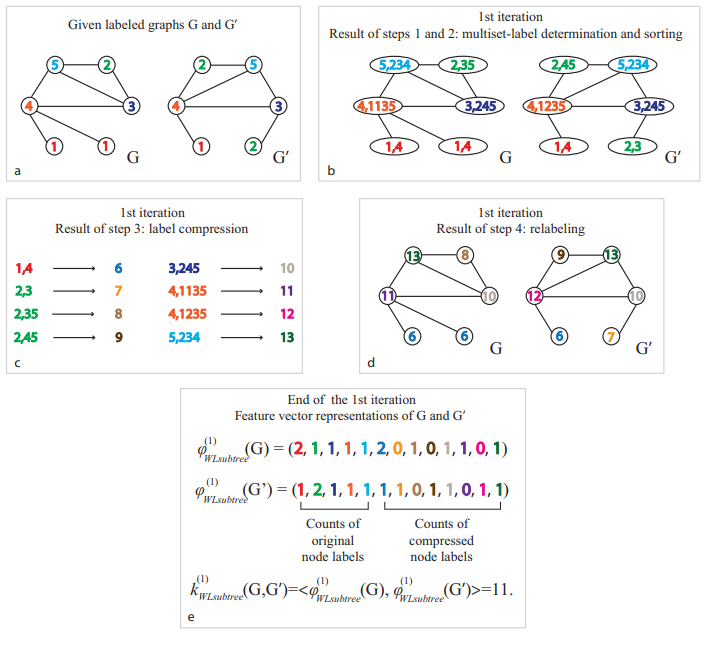
\includegraphics[height=2cm]{fig1.png}
		\end{figure} \pause

	\item Therefore a "fair" clustering must take into account not just the position of the centers, but also the assignment function!

\end{itemize}

\end{frame}

%---------------------------------------------------------


%---------------------------------------------------------
\begin{frame}
\frametitle{Balance}

\begin{block}{Lemma 2(Combination)}
Let $Y, Y' \subset X$ be disjoint.\\
If $\mathcal{C}$ and $\mathcal{C}'$ are clusterings of $Y$ and $Y'$, respectively, then
$$\balance(\mathcal{C} \cup \mathcal{C}') = \min(\balance(\mathcal{C}), \balance(\mathcal{C}'))$$
\end{block}

\begin{itemize}
	\item For any clustering $\mathcal{C}$ of $X$, we have $\balance(\mathcal{C}) \leq \balance(X)$.
	\item If $X$ is not perfectly balanced, then no clustering of $X$ can be perfectly balanced.
\end{itemize}

\end{frame}

%---------------------------------------------------------


%---------------------------------------------------------
\begin{frame}
\frametitle{Toward fairlets }

\begin{alertblock}{Definition}
Let $b, r$ be some integers such that $1 \leq b \leq r$ and $\gcd(b, r) = 1$.

\begin{itemize}
	\item A clustering $\mathcal{Y}$ of $X$ is called a {\it $(b, r)-$fairlet decomposition of $X$} if\\
	(i) $\forall Y \in \mathcal{Y} \ |Y| \leq b + r$ and (ii) $\balance(\mathcal{Y}) = b/r = \balance(X)$
	\item Each $Y \in \mathcal{Y}$ is called a {\it $(b, r)-$fairlet}, or simply {\it fairlet}.
\end{itemize}

\end{alertblock} \pause

\begin{itemize}
	\item Fairlet can be thought of as a group of points that are fair and cannot be split further into true subsets that are also fair.
		\begin{figure}[hbt]
  			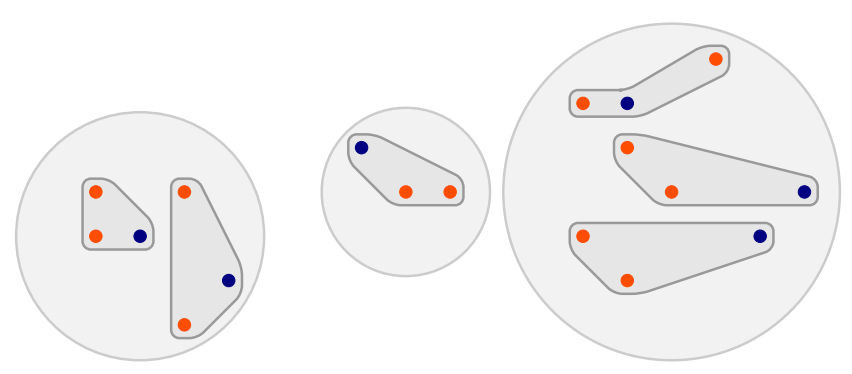
\includegraphics[height=2.5cm]{fig2.png}
		\end{figure} \pause
	\item Intuitively, the balance of the original set of points is preserved while keeping each cluster "small".
\end{itemize}

\end{frame}

%---------------------------------------------------------

%---------------------------------------------------------
\begin{frame}
\frametitle{Toward fairlets}

\begin{block}{Lemma 3}
Let $\balance(X) = b/r$ for some integers $1 \leq b \leq r$ such that $\gcd(b, r) = 1$.

Then there exists a $(b, r)-$fairlet decomposition of $X$.
\end{block} \pause

\begin{itemize}
	\item This lemma tells us that every fair solution to the clustering problem induces a set of minimal fairlets
	\item (Proof is very simple! The proof in the paper seems too complex...)
\end{itemize}

\end{frame}

%---------------------------------------------------------


%---------------------------------------------------------
\begin{frame}
\frametitle{$(t, k)-$fair clustering problems}

\begin{alertblock}{$(t, k)-$fair center (resp. median) problem}
Partition $X$ into $\mathcal{C}$ such that
	\begin{itemize}
		\item $|\mathcal{C}| = k$
		\item $\balance(\mathcal{C}) \geq t$
		\item $\phi(X, \mathcal{C})$ (resp. $\psi(X, \mathcal{C})$) is minimized.
	\end{itemize}
\end{alertblock} \pause

\begin{itemize}
	\item If fairness is not taken into account, the assignment function is implicit through a set $\{c_1, \dots, c_k\}$ of centers i.e.
	$$\alpha(x) = \argmin_{i \in [k]} d(x, c_i)$$ \pause
	\item With fairness, an explicit assignment function is required.
\end{itemize}

\end{frame}

%---------------------------------------------------------

\section{Fairlet decomposition and fair clustering}

%---------------------------------------------------------
\begin{frame}
\frametitle{Fairlet decomposition cost}

\begin{itemize}
	\item $\mathcal{Y} = \{ Y_1, \dots, Y_m \}$: a fairlet decomposition of $X$
	\item $y_j \in Y_j$ is the {\it center} of $Y_j$. (Its choice is arbitrary)
	\item $\beta : X \rightarrow [m]$ is the mapping from a point to the index of the fairlet to which it is mapped.
\end{itemize}

\begin{block}{Definition}
For a fairlet decomposition $\mathcal{Y}$, define its costs:

\begin{itemize}
	\item $k \text{-median cost} = \sum_{x \in X} d \left(x, y_{\beta(x)}\right) =: \psi(X, \mathcal{Y})$
	\item $k \text{-center cost} = \max_{x \in X} d \left(x, y_{\beta(x)}\right) =: \phi(X, \mathcal{Y})$
\end{itemize}

Also, we say that a $(b, r)$-fairlet decomposition is {\it optimal} if it has minimum cost among all possible $(b, r)$-fairlet decompositions.
\end{block}

\end{frame}

%---------------------------------------------------------


%---------------------------------------------------------
\begin{frame}
\frametitle{Reduction to colorblind clustering}

\begin{itemize}
	\item Recall that a $(t, k)$-fair clustering of $X$ requires that $t \leq \balance(X)$ \pause
	
	\item To achieve this, we consider the vanilla $k$-clustering of the \alert{centers of each fairlet} i.e. $k$-clustering of $\{y_1, \dots, y_m\}$ \pause
	
	\item Then we obtain a set of centers $\{c_1, \dots, c_k\}$ and an assignment function $\alpha_Y : Y \rightarrow [k]$. \pause
	
	\item Define $\alpha(x) = \alpha_Y(y_{\beta(x)})$ as the overall assignment function and denote $\mathcal{C}_\alpha$ as the clustering induced by $\alpha$. \pause
	
	\item Then we have that $\balance{C_\alpha} = t$ \pause
	
	\item Also, its cost is bounded, as shown in the next lemma.
\end{itemize}

\end{frame}

%---------------------------------------------------------


%---------------------------------------------------------
\begin{frame}
\frametitle{Reduction to colorblind clustering}

\begin{block}{Lemma 6 (corrected)}
Denote $\tilde{Y}$ as a multiset where each $y_i$ appears $|Y_i|$ number of times. Then,

$$\psi(X, \mathcal{C}_\alpha) \leq \psi(X, \mathcal{Y}) + \psi(\tilde{Y}, \mathcal{C}_\alpha)$$

$$\phi(X, \mathcal{C}_\alpha) \leq \phi(X, \mathcal{Y}) + \phi(\tilde{Y}, \mathcal{C}_\alpha)$$

\end{block} \pause

This lemma, along with previous reasoning, shows that the fair clustering problem can be reduced to
\begin{itemize}
	\item Find a good fairlet decomposition ($\alpha$-approximation)
	\item Solve the vanilla clustering problem on the centers of the fairlets ($\beta$-approximation)
\end{itemize}
, which is actually a $(\alpha + \beta)$-approximation in total!

\end{frame}

%---------------------------------------------------------

\section{Algorithms}

%---------------------------------------------------------

\subsection{(1, k)-fair center problem}

%---------------------------------------------------------
\begin{frame}
\frametitle{Fair $k$-center: $(1, 1)$-fairlets}

\begin{itemize}
	\item Let us first consider the case when $\balance(X) = 1$. \pause
	
	\item How can we find a perfectly balanced clustering? \pause
	
	\item We utilize a good $(1, 1)$-fairlet decomposition! \pause
\end{itemize}

\begin{block}{Lemma 7}
An optimal $(1, 1)$-fairlet decomposition for $k$-center can be found in polynomial time.

\end{block}
{\it (The approach used in the proof will be used later!)}

\end{frame}

%---------------------------------------------------------
\begin{frame}
\frametitle{Proof of Lemma 7}

\begin{itemize}
	\item We shall prove this by relating it to a {\it graph covering problem}.
	
	\item Denote $B(X) = \{b_i\}_i$ and $R(X) = \{r_j\}_j$
	
	\item Create a weighted, {\it complete} bipartite graph $G = (B, R, E)$ with the weight function $w(b_i, r_j) = d(b_i, r_j)$
	
	\item Every $(1, 1)$-fairlet decomposition corresponds to some \alert{perfect matching} in $G$ where each edge represents a fairlet, $Y_i$.
	
	\item Letting $\mathcal{Y} = \{Y_i\}_i$, the $k$-center cost $\phi(X, \mathcal{Y})$ is exactly the cost of the maximum weight edge in the matching.
\end{itemize}

\end{frame}

%---------------------------------------------------------


%---------------------------------------------------------
\begin{frame}
\frametitle{Proof of Lemma 7}

\begin{itemize}
	\item Now, our problem is to find a perfect matching that minimizes the weight of the maximum edge.
	
	\item Can be done in $O(n^2)$ time.\\
	(cf. "threshold graph", binary searching)	
	
	\item For each $Y_i$, arbitrarily set one of the two nodes of the corresponding edge as the center, $y_i$.
\end{itemize}

\end{frame}

%---------------------------------------------------------


%---------------------------------------------------------
\begin{frame}
\frametitle{Fair $k$-center: $(1, 1)$-fairlets}
\setbeamerfont{footnote}{size=\tiny}

\begin{itemize}
	\item Any fair solution induces a set of minimal fairlets. (Lemma 3) \pause
	
	\item Thus, the cost of the fairlet decomposition found is at most {\it twice} the cost of an optimal solution to the clustering.
	
	\begin{block}{Lemma 8 (corrected)\cite{Rosner2019}}
	Let $\mathcal{Y}$ be the partition found previously, and let $\phi_t^*$ be the cost of the optimal $(t, k)$-fair center clustering. Then, $\phi(X, \mathcal{Y}) \leq \alert{2} \phi_t^*$.

	\end{block} \pause
	
	\item Let us utilize a result by Gonzalez for $k$-center problem\footfullcite{Gonzalez1985}:
\end{itemize}

\begin{block}{Theorem (Gonzalez, 1985)}
There is an algorithm which, given a $k$-center instance $\mathcal{I}$, produces a $2$-approximation solution to $\mathcal{I}$ in running time $O(kn)$

\end{block}

\end{frame}

%---------------------------------------------------------


%---------------------------------------------------------
\begin{frame}
\frametitle{Fair $k$-center: $(1, 1)$-fairlets}

\begin{block}{Theorem 9 (corrected)}
The algorithm that first finds fairlets and then clusters them is a \alert{$4$-approximation} for the $(1, k)$-fair center problem.

\end{block}

\end{frame}

%---------------------------------------------------------

\subsection{(1/t', k)-fair center problem}

%---------------------------------------------------------
\begin{frame}
\frametitle{Fair $k$-center: $(1, t')$-fairlets}

\begin{itemize}
	\item Now let us consider the case when $\balance(X) = t < 1$. \pause
	
	\item For simplicity, assume that $t = 1/t'$ for some integer $t' > 1$ (as done in the paper) \pause
	
	\item As a generalization of previous argument, we shall transform this problem into a \alert{minimum cost flow problem (MCFP)}.
\end{itemize}

\end{frame}

%---------------------------------------------------------


%---------------------------------------------------------
\begin{frame}
\frametitle{MCFP}

\begin{block}{Definition}
A {\it flow network} is a directed graph $G = (V, E)$ with a source vertex $s \in V$ and a sink vertex $t \in V$,
where each edge $(u, v) \in E$ has capacity $c(u, v) > 0$, flow $f(u, v) \geq 0$ and cost $a(u, v) \in \mathbb{R}$

\end{block}

\begin{block}{Minimum Cost Flow Problem (MCFP)}
{\bf Input}: A flow network $(G = (V, E), s, t, c, a)$ (without the flow), $d$

{\bf Constraints}:
\begin{itemize}
	\item Capacity constraints: $f(u, v) \leq c(u, v)$
	\item Skew symmetry: $f(u, v) = -f(v, u)$
	\item Flow conservation: $\forall u \not= s, t \ \sum_{w \in V} f(u, w) = 0$
	\item Required flow from $s$ to $t$: $\sum_{w \in V} f(s, w) = \sum_{w \in V} f(w, t) = d$
\end{itemize}

{\bf Output}: Flow $f(u, v)$ such that $\sum_{(u, v) \in E} a(u, v) f(u, v)$ is minimized

\end{block}

\end{frame}

%---------------------------------------------------------


%---------------------------------------------------------
\begin{frame}
\frametitle{Fair $k$-center: $(1, t')$-fairlets}

\begin{itemize}
	\item Let us construct an instance of MCFP, with a parameter $\tau > 0$. \pause
	
	\item First, let us construct a directed graph $H_\tau = (V, E)$ \pause
	
	\item Vertex set:
$$V = \{\beta, \rho\} \cup B(X) \cup R(X) \cup \left\{ b_i^j | b_i \in B(X) \right\}_{j \in [t']} \cup \left\{ r_i^j | r_i \in R(X) \right\}_{j \in [t']}$$ \pause

	\item Edge set:
	\begin{itemize}
		\item $(\beta, \rho)$ with cost 0 and capacity $\min \left( |B(X)|, |R(X)| \right)$
		\item $(\beta, b_i)$ and $(r_i, \rho)$ for each $b_i \in B(X), r_i \in R(X)$, each with cost $0$ and capacity $t' - 1$
		\item $(b_i, b_i^j)$ and $(r_i, r_i^j)$ for each $b_i \in B(X), r_i \in R(X), j \in [t']$, each with cost $0$ and capacity $1$
		\item $(b_i^k, r_j^l)$ for each $b_i \in B(X), r_i \in R(X), 1 \leq k, l \leq t'$, each with cost $1$ if $d(b_i, r_j) \leq \tau$ and $\infty$ otherwise.
	\end{itemize}
	
\end{itemize}

\end{frame}

%---------------------------------------------------------


%---------------------------------------------------------
\begin{frame}
\frametitle{Fair $k$-center: $(1, t')$-fairlets}

\begin{itemize}
	\item To finish the description, we need specify the supply and demand at every node:
	\begin{itemize}
		\item Every node in $B(X)$ has a supply of $1$
		\item Every node in $R(X)$ has a demand of $1$
		\item $\beta$ has a supply of $|R(X)|$
		\item $\rho$ has a demand of $|B(X)|$
		\item Every other node has zero supply and demand
	\end{itemize}
\end{itemize} \pause

\begin{figure}[hbt]
  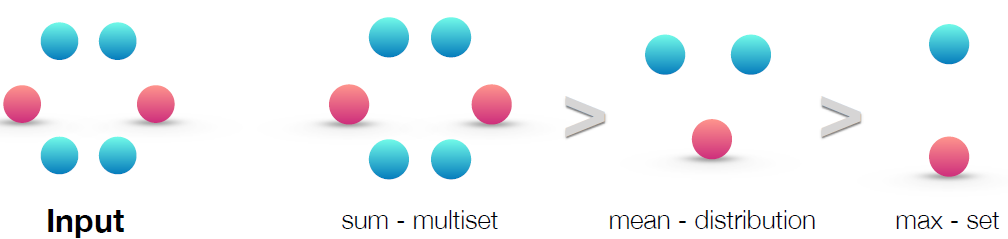
\includegraphics[height=4cm]{fig3.png}
\end{figure}

\end{frame}

%---------------------------------------------------------

%---------------------------------------------------------
\begin{frame}
\frametitle{Fair $k$-center: $(1, t')$-fairlets}

\begin{block}{Lemma 10}
Let $\mathcal{Y}$ be a $(1, t')$-fairlet decomposition of cost $C$ for the $(1/t', k)$-fair center problem. Then it is possible to construct a feasible solution of cost $2C$ to the (constructed) MCF instance.

\end{block}

Above lemma tells us that a $(1, t')$-fairlet decomposition can be used to construct a feasible solution for the MCF instance of twice the cost.

\end{frame}

%---------------------------------------------------------

%---------------------------------------------------------
\begin{frame}
\frametitle{Fair $k$-center: $(1, t')$-fairlets}

\begin{block}{Lemma 11}
Let $\mathcal{Y}$ be an optimal solution of cost $C$ to the (constructed) MCF instance. Then it is possible to construct a $(1, t')$-fairlet decomposition for the $(1/t', k)$-fair center problem of cost at most $C$.

\end{block}

Above lemma tells us that an optimal solution for the MCF instance can be used to obtain a $(1, t')$-fairlet decomposition of bounded cost.

\end{frame}

%---------------------------------------------------------

%---------------------------------------------------------
\begin{frame}
\frametitle{Fair $k$-center: $(1, t')$-fairlets}

Combining the previous two lemmas yield:
 
\begin{block}{Lemma 12}
By reducing the $(1, t')$-fairlet decomposition problem to an MCFP, it is possible to compute a $2$-approximation for the optimal $(1, t')$-fairlet decomposition for the $(1/t', k)$-fair center problem.
\end{block}

Combining above with the result by Gonzalez gives... (next slide)

\end{frame}

%---------------------------------------------------------


%---------------------------------------------------------
\begin{frame}
\frametitle{Fair $k$-center}

\begin{block}{Theorem 13}
For any integer $t' \in \mathbb{N}$, the algorithm that first finds fairlets and then clusters them is a \alert{$4$-approximation} for the $(1/t', k)$-fair center problem.

\end{block}

\end{frame}

%---------------------------------------------------------

\subsection{(1/t', k)-fair median problem}

%---------------------------------------------------------
\begin{frame}
\frametitle{Fair $k$-median}
\setbeamerfont{footnote}{size=\tiny}

\begin{itemize}
	\item Slight modification of previous argument gives us the (approx.) solution for $(t, k)$-fair median problem (with $t = 1/t'$) \pause
	
	\item For the perfectly balanced case, our goal is to look for a \alert{perfect matching of minimum total cost} on the bichromatic graph. \pause
	
	\item To find $(1, t')$-fairlet decomposition for $t' > 1$, create an instance of MCF, {\it with (some of the) weights as the distances}. \pause
	
	\item Let us utilize a result by Li \& Svensson for $k$-median problem\footfullcite{Li2013}:
\end{itemize}

\begin{block}{Theorem (Li \& Svensson, 2013)}
There is an algorithm which, given a $k$-median instance $\mathcal{I}$ and $\varepsilon > 0$, produces a $(1 + \sqrt{3} + \varepsilon)$-approximation solution to $\mathcal{I}$ in running time $O \left( n^{O(1 / \varepsilon^2)} \right)$

\end{block}

\end{frame}

%---------------------------------------------------------


%---------------------------------------------------------
\begin{frame}
\frametitle{Fair $k$-median}

\begin{block}{Theorem 15}
For any integer $t' \in \mathbb{N}$, the algorithm that first finds fairlets and then clusters them is a \alert{$(t' + 1 + \sqrt{3} + \varepsilon)$-approximation} for the $(1/t', k)$-fair median problem.

\end{block}

\end{frame}

%---------------------------------------------------------

\subsection{Hardness}

%---------------------------------------------------------
\begin{frame}
\frametitle{Hardness}

\begin{itemize}
	\item We now have a theoretical framework and an actual algorithm for solving fair clustering problems. \pause
	
	\item But by taking fairness into account, we have introduced some extra complexity to the classical clustering problems. \pause
	
	\item How bad can it be, right? \pause
	
	\item Well, as the next theorem shows, ensuring fairness actually introduces a computational bottleneck! (and a very narrow one, indeed.) \pause
\end{itemize}

\begin{block}{Theorem 16}
For each fixed $t' \geq 3$,

\begin{itemize}
	\item Finding an optimal $(1, t')$-fairlet decomposition is \alert{NP-hard}.
	\item Finding the minimum cost $(1/t', k)$-fair median clustering is \alert{NP-hard}
\end{itemize}

\end{block}

\end{frame}

%---------------------------------------------------------

\section{Experiments}

%---------------------------------------------------------
\begin{frame}
\frametitle{Experiments}

The goal of the experiments is two-fold: \pause

\begin{itemize}
	\item Show that the traditional algorithms for $k$-center and $k$-median tend to produce unfair clusters \pause

	\item Show that the proposed algorithm outputs clusters that respect the fairness guarantees
\end{itemize}

\end{frame}

%---------------------------------------------------------


%---------------------------------------------------------
\begin{frame}
\frametitle{Experiment Design}
\setbeamerfont{footnote}{size=\tiny}

\begin{itemize}
	\item Datasets used: {\bf Diabetes, Bank, Sensus}\footfullcite{Lichman2013}\\
	(Protected attributes: {\bf gender, married or not, gender}, respectively) \pause
	
	\item Flow-based fairlet decomposition algorithm (as proposed) was implemented. \pause
	
	\item For the vanilla $k$-center clustering algorithm, the {\it greedy furthest point algorithm\footfullcite{Gonzalez1985}} was used.\\
	{\small (known to obtain 2-approximation)} \pause
	
	\item For the vanilla $k$-median clustering algorithm, {\it single swap algorithm\footfullcite{Arya2004}} was used.\\
	{\small (known to obtain 5-approximation in the worst case, but performs well in practice. Refer to Kanungo {\it et al.}, 2002)}

\end{itemize}

\end{frame}

%---------------------------------------------------------


%---------------------------------------------------------
\begin{frame}
\frametitle{Results}

In all cases, the experiment was done with $t' = 2$ i.e. aiming for balance of at least $0.5$ in each cluster.

\begin{figure}[hbt]
  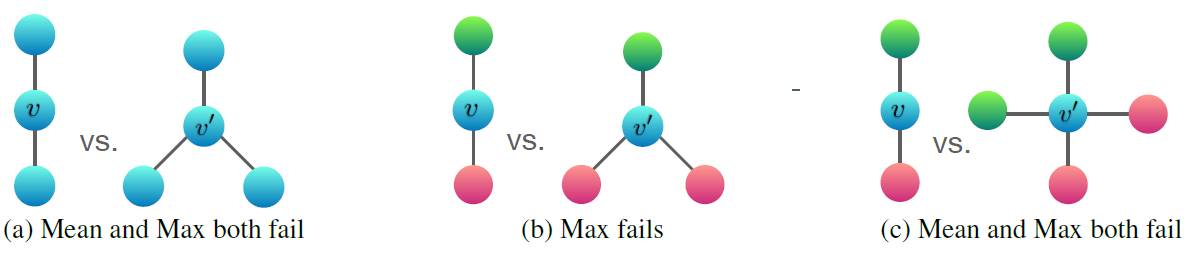
\includegraphics[height=5.5cm]{fig4.png}
\end{figure}

\end{frame}

%---------------------------------------------------------

\section{Summary / Future Research}

%---------------------------------------------------------
\begin{frame}
\frametitle{Summary}

In summary, \pause

\begin{itemize}
	\item Reduction of fair clustering to classical clustering via fairlets \pause

	\item Efficient approximation algorithms for finding fairlet decompositions \pause

	\item Showed that fairness can introduce a computational bottleneck
\end{itemize}

\end{frame}

%---------------------------------------------------------

%---------------------------------------------------------
\begin{frame}
\frametitle{Future research}

\begin{itemize}
	\item Improve the approximation ratio of the decomposition algorithms \pause
	\item Give stronger hardness results \pause
	\item Extend to the case where the protected class is not binary, but can take on multiple values \\
	(Already done! {\it Scalable Fair Clustering (ICML 2019)})
\end{itemize}

\end{frame}

%---------------------------------------------------------

\section{Summary of Fairness}

%---------------------------------------------------------
\begin{frame}
\frametitle{Summary of Fairness}
\setbeamerfont{footnote}{size=\tiny}

Here is a summary of "major" concepts in fairness\footfullcite{Mehrabi2019}\footfullcite{Zhong2019}: (next page)

\end{frame}

%---------------------------------------------------------
\begin{frame}
\frametitle{Summary of Fairness}

\begin{figure}[hbt]
  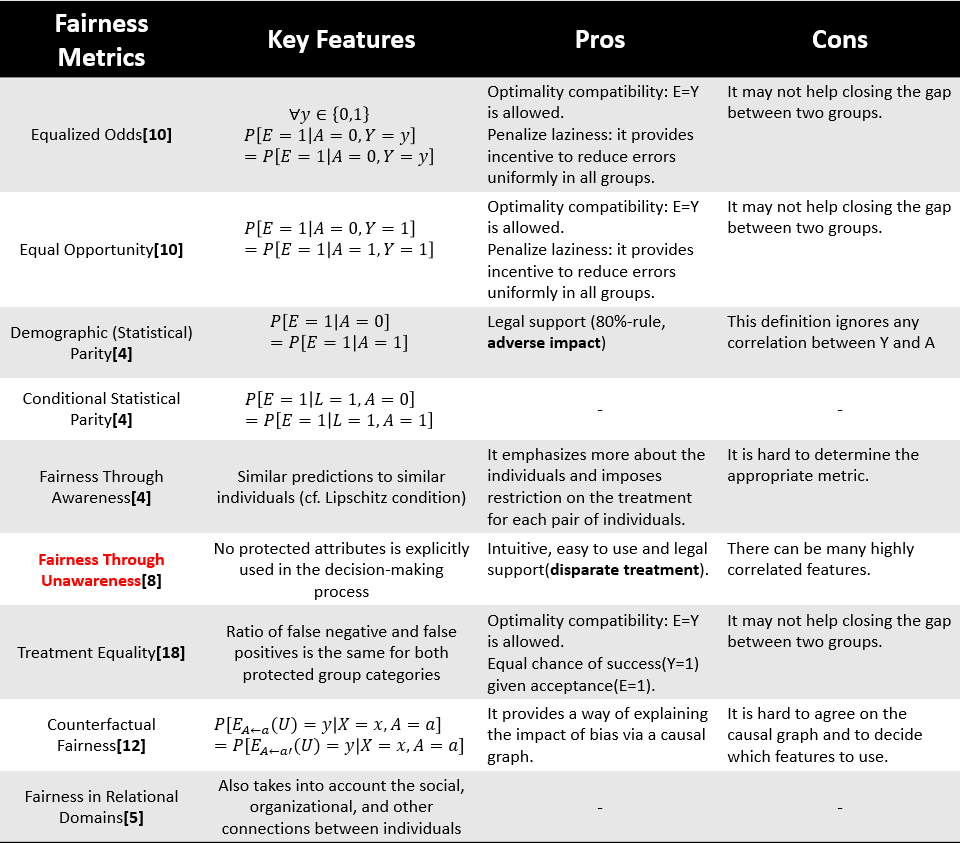
\includegraphics[width=0.7\textwidth]{table.png}
\end{figure}
\end{frame}

%---------------------------------------------------------

\section{References}

%---------------------------------------------------------

\begin{frame}[allowframebreaks]
\frametitle{References}
\nocite{*}
\printbibliography
\end{frame}

%---------------------------------------------------------

\begin{frame}{}
  \centering \Large
  \emph{Thank you for your attention! Any questions?}
\end{frame}

%---------------------------------------------------------

\end{document}